\documentclass[border=4pt]{standalone}
\usepackage{amssymb}
\usepackage{tikz}
\usetikzlibrary{arrows.meta,positioning,shapes.geometric,fit,calc,automata,trees}
\usepackage{float}
\usepackage{booktabs}
\usepackage{longtable}
\usepackage{array}
\usepackage[utf8]{inputenc}
\begin{document}

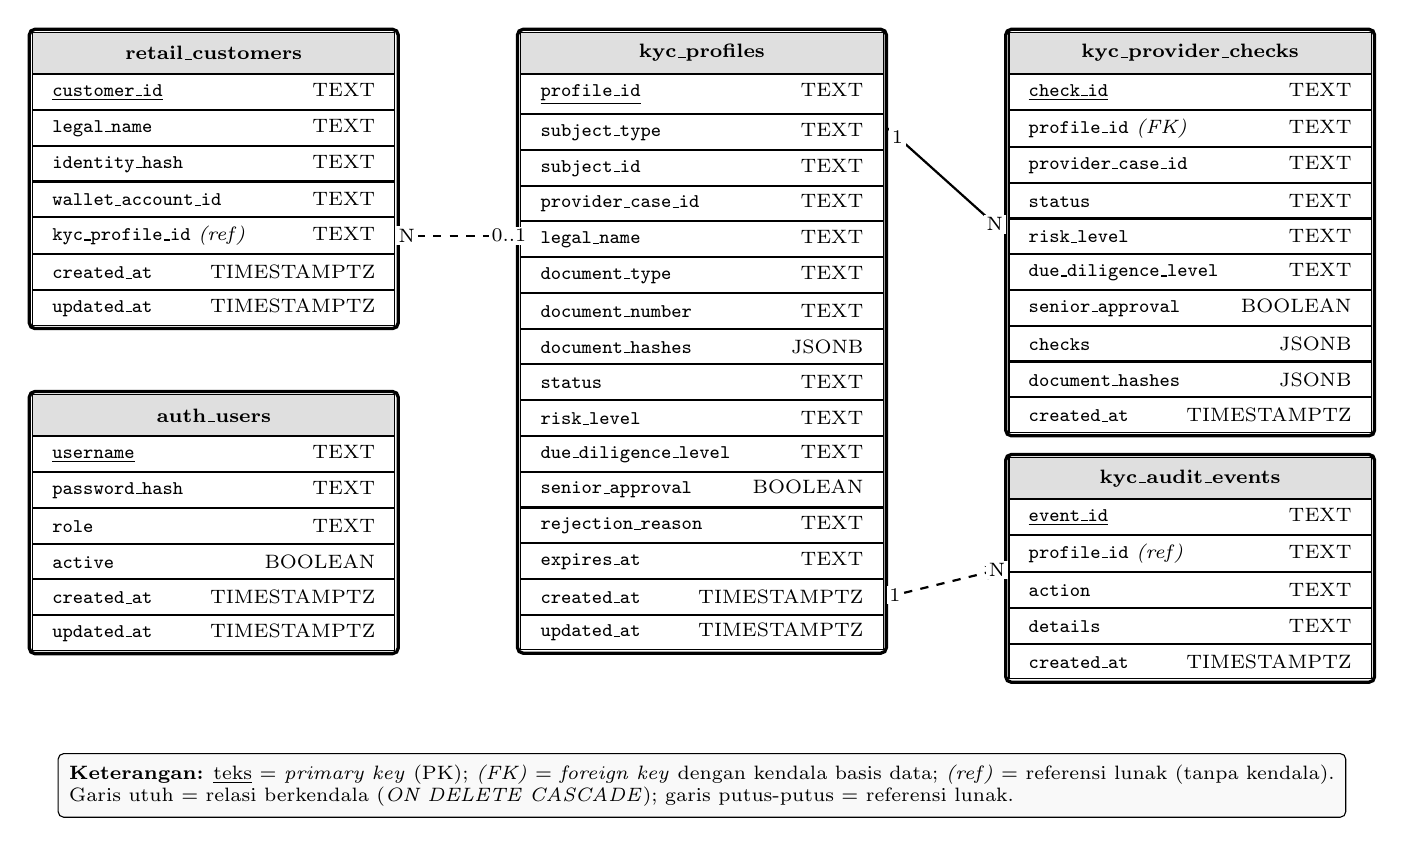
\begin{tikzpicture}[
  ehdr/.style={draw=black, fill=gray!25, rectangle, minimum width=4.6cm,
    minimum height=0.52cm, align=center, font=\scriptsize\bfseries, inner sep=2pt},
  erow/.style={draw=black, fill=white, rectangle, minimum width=4.6cm,
    minimum height=0.44cm, align=left, text width=4.1cm, font=\scriptsize, inner sep=3pt},
  ebox/.style={draw=black, very thick, rounded corners=2pt, inner sep=1pt},
  rel/.style={-{Stealth}, thick},
  soft/.style={-{Stealth}, thick, dashed},
  card/.style={font=\scriptsize, fill=white, inner sep=1pt},
]

%==================== KOLOM TENGAH: kyc_profiles (hub) ====================
\node[ehdr] (ph) at (6.2,0) {kyc\_profiles};
\node[erow, below=0pt of ph]  (p1)  {\underline{\texttt{profile\_id}} \hfill TEXT};
\node[erow, below=0pt of p1]  (p2)  {\texttt{subject\_type} \hfill TEXT};
\node[erow, below=0pt of p2]  (p3)  {\texttt{subject\_id} \hfill TEXT};
\node[erow, below=0pt of p3]  (p4)  {\texttt{provider\_case\_id} \hfill TEXT};
\node[erow, below=0pt of p4]  (p5)  {\texttt{legal\_name} \hfill TEXT};
\node[erow, below=0pt of p5]  (p6)  {\texttt{document\_type} \hfill TEXT};
\node[erow, below=0pt of p6]  (p7)  {\texttt{document\_number} \hfill TEXT};
\node[erow, below=0pt of p7]  (p8)  {\texttt{document\_hashes} \hfill JSONB};
\node[erow, below=0pt of p8]  (p9)  {\texttt{status} \hfill TEXT};
\node[erow, below=0pt of p9]  (p10) {\texttt{risk\_level} \hfill TEXT};
\node[erow, below=0pt of p10] (p11) {\texttt{due\_diligence\_level} \hfill TEXT};
\node[erow, below=0pt of p11] (p12) {\texttt{senior\_approval} \hfill BOOLEAN};
\node[erow, below=0pt of p12] (p13) {\texttt{rejection\_reason} \hfill TEXT};
\node[erow, below=0pt of p13] (p14) {\texttt{expires\_at} \hfill TEXT};
\node[erow, below=0pt of p14] (p15) {\texttt{created\_at} \hfill TIMESTAMPTZ};
\node[erow, below=0pt of p15] (p16) {\texttt{updated\_at} \hfill TIMESTAMPTZ};
\node[ebox, fit=(ph)(p16)] (PROF) {};

%==================== KOLOM KIRI: retail_customers ====================
\node[ehdr] (rh) at (0,0) {retail\_customers};
\node[erow, below=0pt of rh] (r1) {\underline{\texttt{customer\_id}} \hfill TEXT};
\node[erow, below=0pt of r1] (r2) {\texttt{legal\_name} \hfill TEXT};
\node[erow, below=0pt of r2] (r3) {\texttt{identity\_hash} \hfill TEXT};
\node[erow, below=0pt of r3] (r4) {\texttt{wallet\_account\_id} \hfill TEXT};
\node[erow, below=0pt of r4] (r5) {\texttt{kyc\_profile\_id} \textit{(ref)} \hfill TEXT};
\node[erow, below=0pt of r5] (r6) {\texttt{created\_at} \hfill TIMESTAMPTZ};
\node[erow, below=0pt of r6] (r7) {\texttt{updated\_at} \hfill TIMESTAMPTZ};
\node[ebox, fit=(rh)(r7)] (RETAIL) {};

%==================== KOLOM KIRI BAWAH: auth_users (terisolasi) ====================
\node[ehdr] (uh) at (0,-4.6) {auth\_users};
\node[erow, below=0pt of uh] (u1) {\underline{\texttt{username}} \hfill TEXT};
\node[erow, below=0pt of u1] (u2) {\texttt{password\_hash} \hfill TEXT};
\node[erow, below=0pt of u2] (u3) {\texttt{role} \hfill TEXT};
\node[erow, below=0pt of u3] (u4) {\texttt{active} \hfill BOOLEAN};
\node[erow, below=0pt of u4] (u5) {\texttt{created\_at} \hfill TIMESTAMPTZ};
\node[erow, below=0pt of u5] (u6) {\texttt{updated\_at} \hfill TIMESTAMPTZ};
\node[ebox, fit=(uh)(u6)] (AUTH) {};

%==================== KOLOM KANAN ATAS: kyc_provider_checks ====================
\node[ehdr] (ch) at (12.4,0) {kyc\_provider\_checks};
\node[erow, below=0pt of ch]  (c1)  {\underline{\texttt{check\_id}} \hfill TEXT};
\node[erow, below=0pt of c1]  (c2)  {\texttt{profile\_id} \textit{(FK)} \hfill TEXT};
\node[erow, below=0pt of c2]  (c3)  {\texttt{provider\_case\_id} \hfill TEXT};
\node[erow, below=0pt of c3]  (c4)  {\texttt{status} \hfill TEXT};
\node[erow, below=0pt of c4]  (c5)  {\texttt{risk\_level} \hfill TEXT};
\node[erow, below=0pt of c5]  (c6)  {\texttt{due\_diligence\_level} \hfill TEXT};
\node[erow, below=0pt of c6]  (c7)  {\texttt{senior\_approval} \hfill BOOLEAN};
\node[erow, below=0pt of c7]  (c8)  {\texttt{checks} \hfill JSONB};
\node[erow, below=0pt of c8]  (c9)  {\texttt{document\_hashes} \hfill JSONB};
\node[erow, below=0pt of c9]  (c10) {\texttt{created\_at} \hfill TIMESTAMPTZ};
\node[ebox, fit=(ch)(c10)] (CHECK) {};

%==================== KOLOM KANAN BAWAH: kyc_audit_events ====================
\node[ehdr] (ah) at (12.4,-5.4) {kyc\_audit\_events};
\node[erow, below=0pt of ah] (a1) {\underline{\texttt{event\_id}} \hfill TEXT};
\node[erow, below=0pt of a1] (a2) {\texttt{profile\_id} \textit{(ref)} \hfill TEXT};
\node[erow, below=0pt of a2] (a3) {\texttt{action} \hfill TEXT};
\node[erow, below=0pt of a3] (a4) {\texttt{details} \hfill TEXT};
\node[erow, below=0pt of a4] (a5) {\texttt{created\_at} \hfill TIMESTAMPTZ};
\node[ebox, fit=(ah)(a5)] (AUDIT) {};

%==================== RELASI ====================
% kyc_profiles 1 --< N kyc_provider_checks  (FK keras, ON DELETE CASCADE)
\draw[rel] (PROF.east |- c2) -- (CHECK.west)
  node[card, pos=0.08] {1} node[card, pos=0.92] {N};

% kyc_profiles 1 --< N kyc_audit_events  (referensi lunak via profile_id)
\draw[soft] (PROF.east |- p15) -- (AUDIT.west)
  node[card, pos=0.06] {1} node[card, pos=0.94] {N};

% retail_customers N --> 0..1 kyc_profiles  (referensi lunak, nullable)
\draw[soft] (RETAIL.east |- r5) -- (PROF.west |- r5)
  node[card, pos=0.06] {N} node[card, pos=0.94] {0..1};

%==================== LEGENDA ====================
\node[align=left, font=\scriptsize, draw=black, rounded corners=2pt,
  fill=gray!5, inner sep=4pt] at (6.2,-9.3)
  {\textbf{Keterangan:} \underline{teks} = \textit{primary key} (PK);
   \textit{(FK)} = \textit{foreign key} dengan kendala basis data;
   \textit{(ref)} = referensi lunak (tanpa kendala).\\
   Garis utuh = relasi berkendala (\textit{ON DELETE CASCADE});
   garis putus-putus = referensi lunak.};

\end{tikzpicture}%

\end{document}
